% Options for packages loaded elsewhere
\PassOptionsToPackage{unicode}{hyperref}
\PassOptionsToPackage{hyphens}{url}
\PassOptionsToPackage{dvipsnames,svgnames,x11names}{xcolor}
%
\documentclass[
]{article}

\usepackage{amsmath,amssymb}
\usepackage{iftex}
\ifPDFTeX
  \usepackage[T1]{fontenc}
  \usepackage[utf8]{inputenc}
  \usepackage{textcomp} % provide euro and other symbols
\else % if luatex or xetex
  \usepackage{unicode-math}
  \defaultfontfeatures{Scale=MatchLowercase}
  \defaultfontfeatures[\rmfamily]{Ligatures=TeX,Scale=1}
\fi
\usepackage{lmodern}
\ifPDFTeX\else  
    % xetex/luatex font selection
\fi
% Use upquote if available, for straight quotes in verbatim environments
\IfFileExists{upquote.sty}{\usepackage{upquote}}{}
\IfFileExists{microtype.sty}{% use microtype if available
  \usepackage[]{microtype}
  \UseMicrotypeSet[protrusion]{basicmath} % disable protrusion for tt fonts
}{}
\makeatletter
\@ifundefined{KOMAClassName}{% if non-KOMA class
  \IfFileExists{parskip.sty}{%
    \usepackage{parskip}
  }{% else
    \setlength{\parindent}{0pt}
    \setlength{\parskip}{6pt plus 2pt minus 1pt}}
}{% if KOMA class
  \KOMAoptions{parskip=half}}
\makeatother
\usepackage{xcolor}
\ifLuaTeX
  \usepackage{luacolor}
  \usepackage[soul]{lua-ul}
\else
  \usepackage{soul}
  
\fi
\setlength{\emergencystretch}{3em} % prevent overfull lines
\setcounter{secnumdepth}{5}
% Make \paragraph and \subparagraph free-standing
\makeatletter
\ifx\paragraph\undefined\else
  \let\oldparagraph\paragraph
  \renewcommand{\paragraph}{
    \@ifstar
      \xxxParagraphStar
      \xxxParagraphNoStar
  }
  \newcommand{\xxxParagraphStar}[1]{\oldparagraph*{#1}\mbox{}}
  \newcommand{\xxxParagraphNoStar}[1]{\oldparagraph{#1}\mbox{}}
\fi
\ifx\subparagraph\undefined\else
  \let\oldsubparagraph\subparagraph
  \renewcommand{\subparagraph}{
    \@ifstar
      \xxxSubParagraphStar
      \xxxSubParagraphNoStar
  }
  \newcommand{\xxxSubParagraphStar}[1]{\oldsubparagraph*{#1}\mbox{}}
  \newcommand{\xxxSubParagraphNoStar}[1]{\oldsubparagraph{#1}\mbox{}}
\fi
\makeatother


\providecommand{\tightlist}{%
  \setlength{\itemsep}{0pt}\setlength{\parskip}{0pt}}\usepackage{longtable,booktabs,array}
\usepackage{calc} % for calculating minipage widths
% Correct order of tables after \paragraph or \subparagraph
\usepackage{etoolbox}
\makeatletter
\patchcmd\longtable{\par}{\if@noskipsec\mbox{}\fi\par}{}{}
\makeatother
% Allow footnotes in longtable head/foot
\IfFileExists{footnotehyper.sty}{\usepackage{footnotehyper}}{\usepackage{footnote}}
\makesavenoteenv{longtable}
\usepackage{graphicx}
\makeatletter
\def\maxwidth{\ifdim\Gin@nat@width>\linewidth\linewidth\else\Gin@nat@width\fi}
\def\maxheight{\ifdim\Gin@nat@height>\textheight\textheight\else\Gin@nat@height\fi}
\makeatother
% Scale images if necessary, so that they will not overflow the page
% margins by default, and it is still possible to overwrite the defaults
% using explicit options in \includegraphics[width, height, ...]{}
\setkeys{Gin}{width=\maxwidth,height=\maxheight,keepaspectratio}
% Set default figure placement to htbp
\makeatletter
\def\fps@figure{htbp}
\makeatother
% definitions for citeproc citations
\NewDocumentCommand\citeproctext{}{}
\NewDocumentCommand\citeproc{mm}{%
  \begingroup\def\citeproctext{#2}\cite{#1}\endgroup}
\makeatletter
 % allow citations to break across lines
 \let\@cite@ofmt\@firstofone
 % avoid brackets around text for \cite:
 \def\@biblabel#1{}
 \def\@cite#1#2{{#1\if@tempswa , #2\fi}}
\makeatother
\newlength{\cslhangindent}
\setlength{\cslhangindent}{1.5em}
\newlength{\csllabelwidth}
\setlength{\csllabelwidth}{3em}
\newenvironment{CSLReferences}[2] % #1 hanging-indent, #2 entry-spacing
 {\begin{list}{}{%
  \setlength{\itemindent}{0pt}
  \setlength{\leftmargin}{0pt}
  \setlength{\parsep}{0pt}
  % turn on hanging indent if param 1 is 1
  \ifodd #1
   \setlength{\leftmargin}{\cslhangindent}
   \setlength{\itemindent}{-1\cslhangindent}
  \fi
  % set entry spacing
  \setlength{\itemsep}{#2\baselineskip}}}
 {\end{list}}
\usepackage{calc}
\newcommand{\CSLBlock}[1]{\hfill\break\parbox[t]{\linewidth}{\strut\ignorespaces#1\strut}}
\newcommand{\CSLLeftMargin}[1]{\parbox[t]{\csllabelwidth}{\strut#1\strut}}
\newcommand{\CSLRightInline}[1]{\parbox[t]{\linewidth - \csllabelwidth}{\strut#1\strut}}
\newcommand{\CSLIndent}[1]{\hspace{\cslhangindent}#1}

\makeatletter
\@ifpackageloaded{tcolorbox}{}{\usepackage[skins,breakable]{tcolorbox}}
\@ifpackageloaded{fontawesome5}{}{\usepackage{fontawesome5}}
\definecolor{quarto-callout-color}{HTML}{909090}
\definecolor{quarto-callout-note-color}{HTML}{0758E5}
\definecolor{quarto-callout-important-color}{HTML}{CC1914}
\definecolor{quarto-callout-warning-color}{HTML}{EB9113}
\definecolor{quarto-callout-tip-color}{HTML}{00A047}
\definecolor{quarto-callout-caution-color}{HTML}{FC5300}
\definecolor{quarto-callout-color-frame}{HTML}{acacac}
\definecolor{quarto-callout-note-color-frame}{HTML}{4582ec}
\definecolor{quarto-callout-important-color-frame}{HTML}{d9534f}
\definecolor{quarto-callout-warning-color-frame}{HTML}{f0ad4e}
\definecolor{quarto-callout-tip-color-frame}{HTML}{02b875}
\definecolor{quarto-callout-caution-color-frame}{HTML}{fd7e14}
\makeatother
\makeatletter
\@ifpackageloaded{caption}{}{\usepackage{caption}}
\AtBeginDocument{%
\ifdefined\contentsname
  \renewcommand*\contentsname{Table of contents}
\else
  \newcommand\contentsname{Table of contents}
\fi
\ifdefined\listfigurename
  \renewcommand*\listfigurename{List of Figures}
\else
  \newcommand\listfigurename{List of Figures}
\fi
\ifdefined\listtablename
  \renewcommand*\listtablename{List of Tables}
\else
  \newcommand\listtablename{List of Tables}
\fi
\ifdefined\figurename
  \renewcommand*\figurename{Figure}
\else
  \newcommand\figurename{Figure}
\fi
\ifdefined\tablename
  \renewcommand*\tablename{Table}
\else
  \newcommand\tablename{Table}
\fi
}
\@ifpackageloaded{float}{}{\usepackage{float}}
\floatstyle{ruled}
\@ifundefined{c@chapter}{\newfloat{codelisting}{h}{lop}}{\newfloat{codelisting}{h}{lop}[chapter]}
\floatname{codelisting}{Listing}
\newcommand*\listoflistings{\listof{codelisting}{List of Listings}}
\makeatother
\makeatletter
\makeatother
\makeatletter
\@ifpackageloaded{caption}{}{\usepackage{caption}}
\@ifpackageloaded{subcaption}{}{\usepackage{subcaption}}
\makeatother
\ifLuaTeX
  \usepackage{selnolig}  % disable illegal ligatures
\fi
\usepackage{bookmark}

\IfFileExists{xurl.sty}{\usepackage{xurl}}{} % add URL line breaks if available
\urlstyle{same} % disable monospaced font for URLs
\hypersetup{
  pdftitle={Navigating food web prediction; assumptions, rationale, and methods},
  pdfauthor={Tanya Strydom; Jennifer A. Dunne; Timothée Poisot; Andrew P. Beckerman},
  pdfkeywords={food web, network construction, scientific ignorance},
  colorlinks=true,
  linkcolor={blue},
  filecolor={Maroon},
  citecolor={Blue},
  urlcolor={Blue},
  pdfcreator={LaTeX via pandoc}}


\title{Navigating food web prediction; assumptions, rationale, and
methods}
\author{Tanya Strydom %
%
\textsuperscript{%
%
1%
}%
; Jennifer A. Dunne %
%
\textsuperscript{%
%
2%
}%
; Timothée Poisot %
%
\textsuperscript{%
3,%
4%
}%
; Andrew P. Beckerman %
%
\textsuperscript{%
%
1%
}%
}
\date{2024-06-04}

\usepackage{setspace}
\usepackage[left]{lineno}
\usepackage[letterpaper]{geometry}

\usepackage[nolists,noheads,markers]{endfloat}
\geometry{margin=2.5cm}

\begin{document}

\thispagestyle{empty}
{\bfseries\sffamily\Large Navigating food web prediction; assumptions,
rationale, and methods}
\vfil
Tanya Strydom %
%
\textsuperscript{%
%
1%
}%
; Jennifer A. Dunne %
%
\textsuperscript{%
%
2%
}%
; Timothée Poisot %
%
\textsuperscript{%
3,%
4%
}%
; Andrew P. Beckerman %
%
\textsuperscript{%
%
1%
}%

\vfil
{\small
\textbf{Abstract:} TODO
\vfil
\textbf{Keywords:} %
food web, network construction, %
scientific ignorance%
}
\clearpage
\setcounter{page}{1}
\doublespacing
\linenumbers

At the heart of modern biodiversity science are a set of concepts about
biodiversity, community structure, productivity, and asynchrony, and how
they define the stability, resilience, and dynamics of complex
communities. The use of species interaction networks provides a powerful
abstraction that one can use to help quantify, conceptualise, and
understand these concepts. However, network ecology has its own nuance
and idiosyncrasies that not only provide a barrier to entry but causes
dissonance even within the field (Dormann, 2023). This is perhaps
particularly pervasive within the space of network prediction\ldots{}

One of the fundamental challenges that we are faced when working with
and studying interaction networks (and, within the context of this
manuscript, specifically food webs) is that there is a scarcity of `real
world' interaction data (Hortal et al., 2015; Poisot et al., 2021). The
difficulty of recording interactions in the field (Jordano, 2016a,
2016b) has necessitated that researchers find and develop alternative
means to construct and build food webs using \textbf{models}
(Morales-Castilla et al., 2015; Strydom et al., 2021). Over the past
decade, there has been a proliferation of tools and processes for
characterising food webs, these models span a wide range of philosophies
that rely on different approaches, data, and definitions, which
ultimately determine how the food web is constructed and coded. Although
the development of these different models have carved out the path for
constructing either synthetic, ecologically plausible networks (Poisot,
Gravel, et al., 2016), or providing `first draft' networks that can be
utilised in real world settings (Strydom et al., 2022) we are still
lacking in discussions that are explicitly comparing and contrasting how
the way one chooses to approach the task of constructing a food web is
introducing (and ultimately embedding) specific assumptions and
hypotheses (Petchey et al., 2008). Most attempts that focus on comparing
and contrasting models are focused on the same group of \textbf{model
families} (Pichler et al., 2020; Williams \& Martinez, 2008) and only
benchmark the different models as opposed to contextualising them within
the bigger framework of understanding the data needs of the different
models, as well as how the resulting network is defined and structured.
As food webs become a more integrated part of some of the broader fields
of ecology (Bhatia et al., 2023; Thuiller et al., 2024) it is critical
that we review these different model families as a whole (not only in
isolation), and move away from simply benchmarking the performance of
these different model families. This is important because different
models impose different constraints upon themselves and will not only
delimit and dictate the potential questions one will be able to ask
(Petchey et al., 2011) but also determine the appropriate research
setting for which the model (and resulting network) can be used. For
example the use of `structural food webs' are useful for developing
additional theory such as re-wiring of networks (Staniczenko et al.,
2010) but would be meaningless if one's intention is to produce a
location-specific network {[}do we need an \emph{e.g.,} ref??{]}. This
will allow us to ensure the right models are being used to answer the
right questions, particularly within the context of trying to accelerate
cross-cutting research in the face of global change.

When navigating the seas of using and constructing food webs the
researcher needs to be able to clearly articulate and define the
parameters that are used to define their food web(s) of interest. This
will aid them in being able to select the correct model to help them to
reach their goal. In order to be able to make informed decisions it is
important that one has a strong grasp of exactly what it means to
`code'/define a food web (Section~\ref{sec-network-anatomy}), a clear
understanding of why one wants to predict a food web
(Section~\ref{sec-network-why}), and ultimately one needs to be able to
asses and evaluate which model family is going to best match up with the
goal of network prediction (Section~\ref{sec-network-build}). Here we
specifically aim to look at not look at only the performance of the
different models but also initiate a (thus far lacking) discussion
around how the interplay between the language used to define networks
and the underlying theory/philosophy should also be a part of the
broader discussion when it comes to the task of `model selection'.

\begin{figure}

\centering{

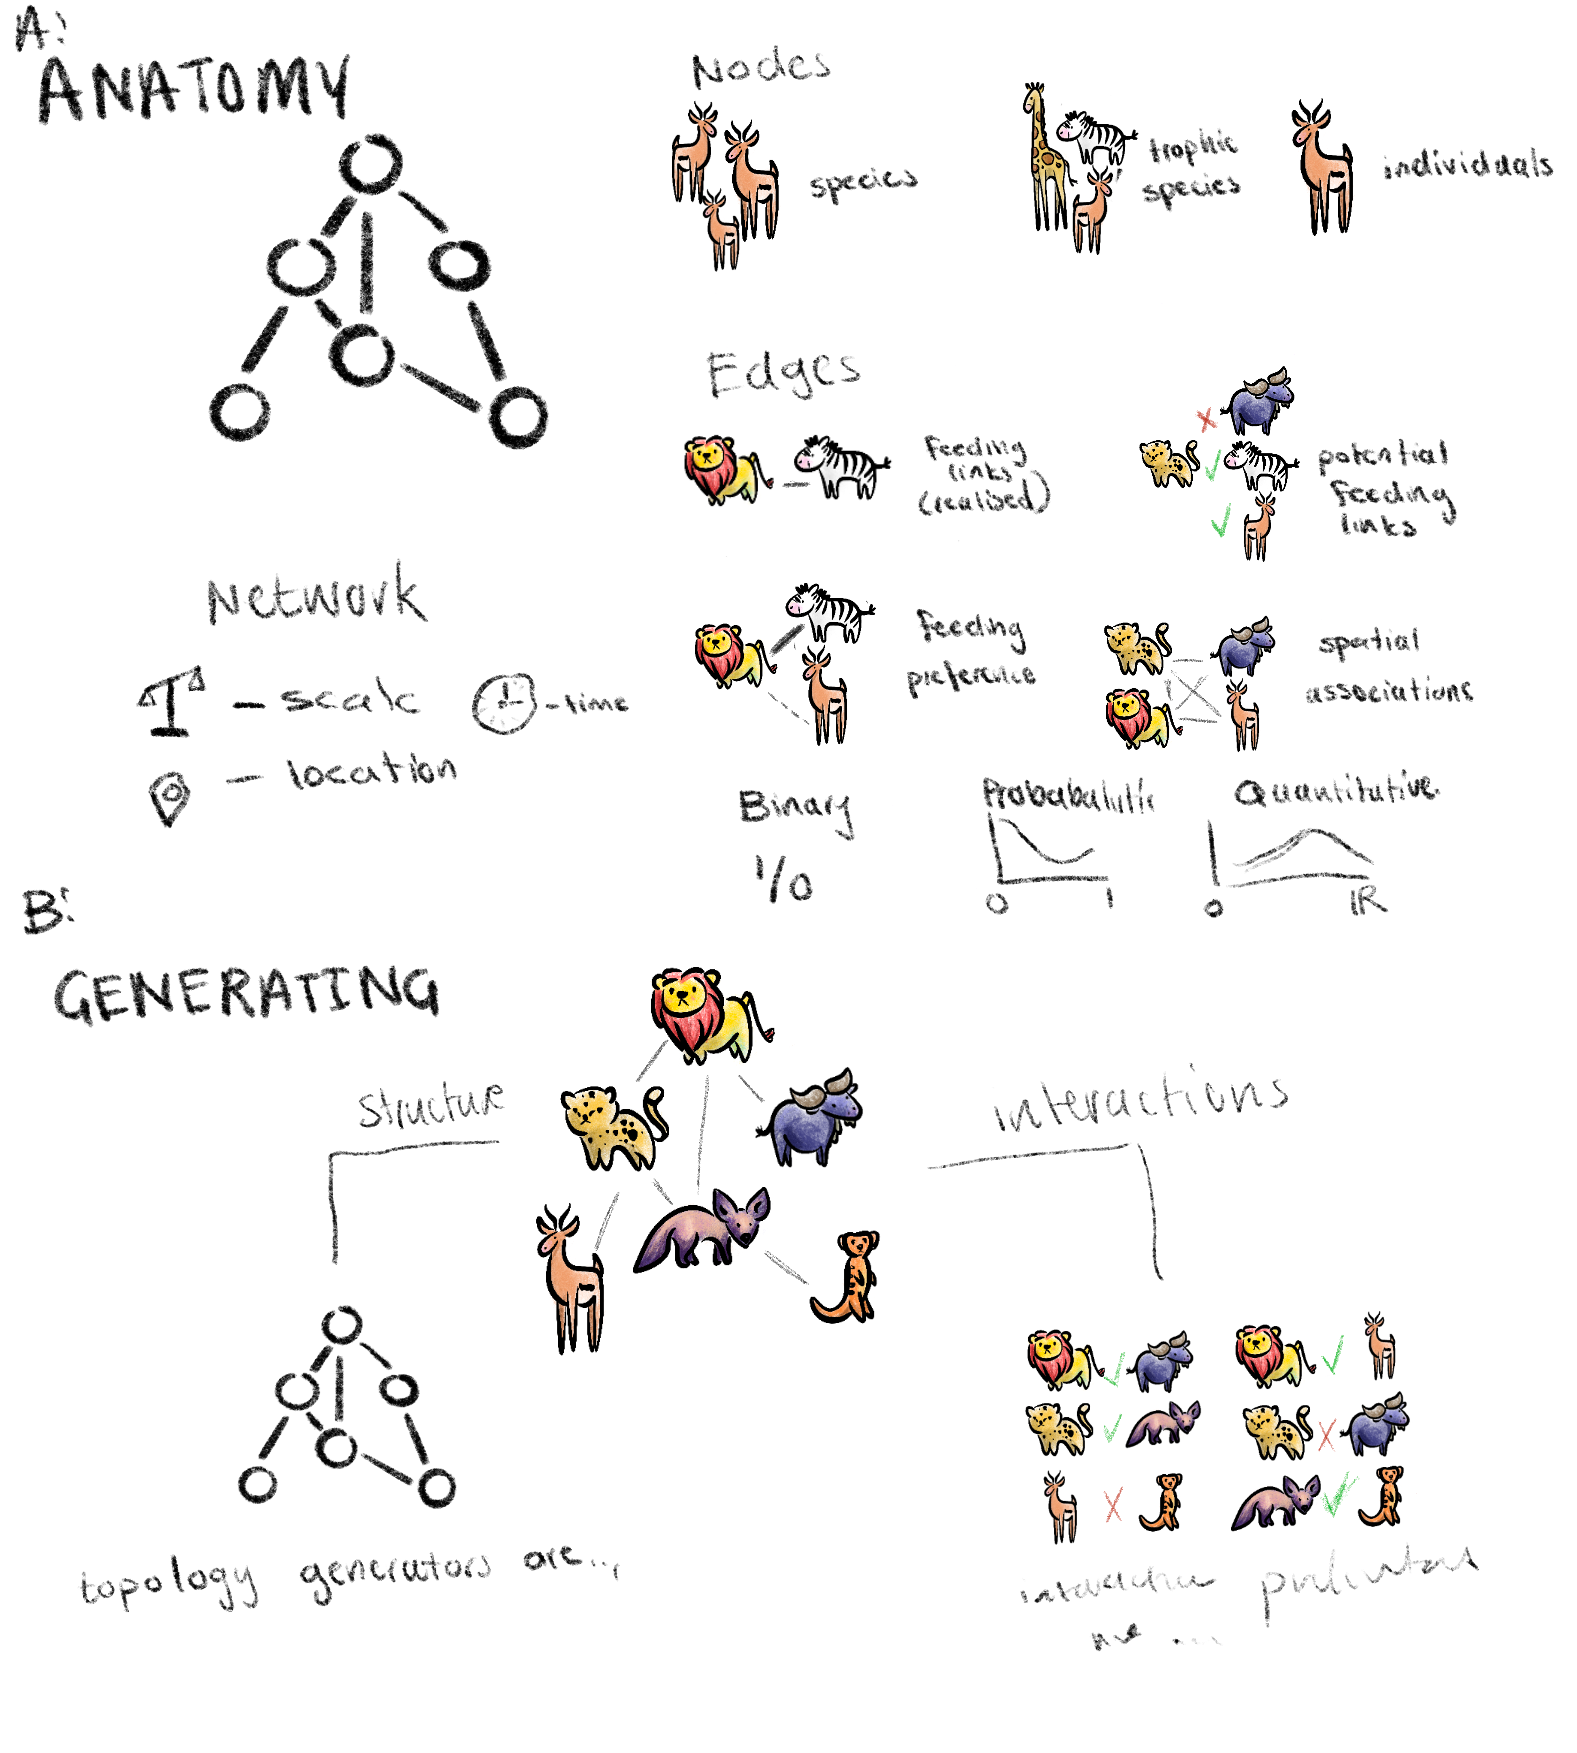
\includegraphics{images/concept_2.png}

}

\caption{\label{fig-concept}Panel \textbf{A} shows the many ways in
which a food web can be defined and described at the node, edge, and
even network level. Panel \textbf{B} (will) shows how the way in which
we predict networks also limited and often focuses only only predicting
the structure of a network (the final networks is parametrised by the
expected structure of the network) or the interactions between species
(the final network is determined by the behaviour of the nodes). These
different models also encode different philosophies/hypotheses not only
as to what determines how a network will look like but also how the
final network itself is encoded \emph{i.e.,} its anatomy. (\emph{aside:}
there is the potential to either try and visually summarise how the
different model families define a network (so repeating the motifs used
in the ANATOMY panel) alternatively it would be cool to try and have a
panel C that tries to quantify the different `data ingredients' you
would need to try and construct a network, this would probably be very
visually overwhelming though\ldots)}

\end{figure}%

\section{The anatomy of a food web}\label{sec-network-anatomy}

Defining a food web seems simple, it is the representation of the
interactions (edges) between species (nodes), however the definition of
`edges' and `nodes', as well as the scale at which they are aggregated
can take many forms. As highlighted in Poisot, Stouffer, et al. (2016)
networks can be constructed at the population (the links among
individuals), community (the links between species), or metacommunity
(fluxes between locations) level. Even if one were to limit their scope
to thinking of interaction networks only in terms of food webs at the
community-level there are still many ways to define the various
components of the network Panel A of~\ref{fig-concept}, one needs to
understand the different intentions/assumptions that are made when a
food web is constructed. Although the main intention of a food web is to
capture and represent the feeding links between species there are many
ways to define the nodes (\emph{e.g.,} species or taxonomic group),
edges (\emph{e.g.,} \textbf{potential} or \textbf{realised feeding
links}), the magnitude of the edges (\emph{e.g.,} binary vs
probabilistic), and even how the network itself is delimited (does it
represent an aggregation of interactions over time?).

\subsection{How do we define a node?}\label{how-do-we-define-a-node}

Although this may seem an elementary question in the context of food
webs --- a node \emph{should} represent a (taxonomic) species, the
reality is that nodes can often represent an aggregation of different
species - so called `trophic species' or segregation of species by life
stages. Representing nodes as non-taxonomic species can be useful in
certain contexts (Williams \& Martinez, 2000) and in cases where the
adult and larval stages of a species have different diets it may make
ecological sense (Clegg et al., 2018) meaning that it is not uncommon
that networks often have nodes that have different definitions of a
`species' \emph{e.g.} consisting of both taxonomic and trophic species.
Practical implications of how we are aggregating the nodes is that the
resolution may not always be `pixel perfect' \emph{i.e.,} we may be
unable to assess the co-extinction risk of a species pair, however there
is value in having nodes that represent an aggregation of species, as
these convey a much more general overview of how the links are
distributed within the community.

\subsection{What is meant by an edge?}\label{what-is-meant-by-an-edge}

As discussed earlier there are many ways to define the links between
species --- even feeding links. At its core links within food webs can
be thought of as a representation of either the flow of a resource
{[}ref{]}, realised (Pringle, 2020) or potential (Dunne, 2006) feeding
links, or energy transfer and material flow (Lindeman, 1942). How we
specify links will influence the resulting structure of the network -
and the inferences we will make thereof. For example taking a food web
that consists of links representing \emph{potential} feeding links
between species will be meaningless if you are interested in
understanding \emph{e.g.,} the flow of energy through the system as the
links within the network are over overrepresented. In addition to the
various ways of defining the links between species pairs there are also
a myriad of ways in which the links themselves can be quantified. Links
between species are often treated as being present or absent
(\emph{i.e.,} binary) but it is also possible to use probabilities
(which quantifies how likely an interaction is to occur, Poisot,
Cirtwill, et al., 2016) or continuous measurements (which quantifies the
strength of of an interaction, Berlow et al., 2004). Moving away from a
purely binary way of representing allows us to quantify a level of
(un)certainty of our knowledge of interactions (\emph{i.e.,} moving from
being able to ask if are they occurring to quantifying how likely they
are to occur) does add an additional level of `complexity' to the
construction and interpretation of networks, but ultimately it allows us
to capture more information at different scales (Banville, in prep).

\subsection{Putting the parts together; what does it
mean?}\label{putting-the-parts-together-what-does-it-mean}

The ingredients one uses to construct networks from nodes and edges
generates a unique representation of the mechanisms (see Box 1 -
Mechanisms that determine feeding links) that allow inference and
reasoning about the structure, aspects of dynamics (\emph{e.g.,}
stability), and potentially the function of communities (\emph{e.g.,}
flux). It is thus beneficial to keep in mind that in the process of
`codifying' a network one is already embedding some sort of hypothesis
as to the nature of the feeding links between species (Brimacombe et
al., 2023; Proulx et al., 2005). Here it may be meaningful to
contextualise the different `types' of food webs within the larger
research programmes (or even practical needs) that have been driving the
construction of them.

\begin{tcolorbox}[enhanced jigsaw, colback=white, breakable, title=\textcolor{quarto-callout-note-color}{\faInfo}\hspace{0.5em}{Box 1 - Mechanisms that determine feeding links}, leftrule=.75mm, opacitybacktitle=0.6, coltitle=black, opacityback=0, rightrule=.15mm, toprule=.15mm, colbacktitle=quarto-callout-note-color!10!white, arc=.35mm, bottomtitle=1mm, bottomrule=.15mm, titlerule=0mm, toptitle=1mm, colframe=quarto-callout-note-color-frame, left=2mm]

There are many ideas as to what are the underlying mechanisms that
determine the links between species. The way one chooses to encode a
network will most likely also be reflective of (or only be able to
encapsulate) one or a few of the different mechanisms. There is probably
even an argument to be had that depending on how we define a network we
will probably expect some of the `hypotheses' of the different
mechanisms to hold. \emph{e.g.,} I think most people will agree that the
feasibility of interactions between specific species pairs is not random
(there needs to be some sort of trait/form complementarity) but how/if
they interact within the environment (\emph{i.e.,} the realisation of
the interactions) \emph{might} as well be (also probably even more
relevant if one thinks about/works with trophic species\ldots)

\textbf{Proximity}

We are co-occurring in space and in time and thus we can interact
(Barberán et al., 2012)

\textbf{Mass-effect}

Our (respective and instantaneous) abundance in that time and space is
going to influence how we interact. \emph{Sensu} Hubbell (2001) Neutral
Theory

\textbf{Complementarity}

We have a set of `traits' that means we can interact including:

\begin{itemize}
\tightlist
\item
  You as a prey item fit in my gob (I can eat you, \st{even if its small
  bites}) {[}ref{]}
\item
  You as a prey item are energetically `worth it' \st{and allowing me to
  hit all the right macros} {[}ref foraging ecology{]}
\item
  As a predator I have the required traits that allow me to \st{kill}
  unalive and eat you (\emph{sensu} forbidden links Jordano, 2016b)
\item
  As predator and prey we have been co-occurring for a long time and I
  have found ways to eat you (trying to capture the idea of evolutionary
  time)
\end{itemize}

\textbf{`Structural'}

The `energy budget' for the environment means that only \(y\) links are
possible between us \(x\) number of species and so our interactions
reflect that. Or is it more the only way we can all access the energy
resource is by arranging ourselves into trophic units\ldots{}

\textbf{None}

We are therefore we interact. This is random.

\end{tcolorbox}

\section{Why do we want to predict food webs?}\label{sec-network-why}

As discussed in Section~\ref{sec-network-anatomy} there are many ways to
define a food web, meaning that there are equally as many reasons one
might be interested in predicting a food web. However we may think of
two primary drivers for wanting to predict networks (Panel B
Figure~\ref{fig-concept}), namely an interest in generating a set of
ecologically plausible networks (\emph{i.e.,} being able to describe
networks using a model) or being able to recover (predict) location
specific, `realised', interactions for a specific species community
(\emph{i.e.,} being able to predict/infer the interactions between
species). Of course these two categories are not distinct, mutually
exclusive, groups but can rather be viewed as operating on a continuum
ranging from a need for generality (\emph{i.e.,} creating a network
that, when taken in aggregate, the distribution of links (interactions)
between nodes (species) are ecologically plausible) to a need for
specificity (\emph{i.e.,} local-level predictions between specific
species pairs). Although the ability to predict `real-world'
interactions (and the resulting food webs) can have more intuitive `real
world' applications \emph{e.g.,} being able to `recover' food webs that
have since gone extinct (Dunne et al., 2008; Yeakel et al., 2014), using
pairwise interactions to understand species distributions (Pollock et
al., 2014) or even co-extinction risk (Dunn et al., 2009), a more
structural approach to network construction affords one an opportunity
to interrogate some of the more high-level mechanisms that are
structuring networks (Box 1).

It is perhaps more important that when one is talking about `why' they
want to predict networks to articulate exactly what anatomical part of
the food web we are interested in scrutinising.

\section{How do we predict food webs?}\label{sec-network-build}

Selecting a model for the task of network prediction should come down to
two things; what \emph{aspect} of a food web one is interested in
predicting, and what data are available, necessary, and sufficient. As
shown in panel B of Figure~\ref{fig-concept} the interest in a network
is (usually) at either the `structural' or `interaction' level and the
development of models for the task of network prediction often focus on
high fidelity (performance) at one of these scales. With this in mind it
is beneficial to think of the different model families relative to these
two different goals; here we refer to models that are used to predict
the structure of a network as \textbf{topology generators} and models
developed to infer the interactions for a given species pool as
\textbf{interaction predictors}. It is meaningful to make this
distinction because although it is possible to construct a food web
given using an \emph{interaction predictor} the models themselves lack
any sort of parametrisation of the network structure and so the
resulting network is a poor reflection of the actual network structure
(Caron et al., 2024). This is primarily because \emph{interaction
predictors} are models that evaluate the feasibility of an interaction
between species pairs and not in the context of feasibility at the
community level. Models themselves are a reflection of the different
goals and intentions of the research program from which they are
developed and are often `described' by a specific mechanism that will
determine the resulting structure or interactions (Box 1). Models such
as the niche (Williams \& Martinez, 2000) or cascade (Cohen et al.,
1990) were developed with the intent of being used to understand the
\emph{structural} aspects of food webs, specifically how links are
distributed amongst species in the community, whereas bayesian (Cirtwill
et al., 2019) or trait hierarchy (Shaw et al., 2024) models have been
developed on the basis that the traits of a species are the underlying
mechanism in determining the feasibility of interactions (\emph{i.e.,}
species \(a\) has the capacity to eat species \(b\)). Along with
predicting different anatomical parts of a food web the different models
have varying degrees of data that are needed to `parametrise' the
network. Once these two limitations are assessed and addressed it is
then possible to select the model (or model family) that will best be
able to capture food web feature that the researcher is most interested
in (see Box 2 - Assessing model outputs). It is thus clear that
(realistically) there will probably never be a `best fit' tool that is
able to construct a food web that will span the entire range of needs,
and rather the responsibility lies with the researcher to be aware of
not only the underlying philosophy of the specific toolset (as this
could have knock-on effects when using those networks for downstream
analyses/simulations; pers. comms. Beckerman, 2024), but also how well
the tool is able to retrieve the specific network or interaction
properties that is of interest.

\begin{quote}
In order for a model to formalise a `complete' food web it is necessary
to formalise two aspects of the network, `who eats whom' (to determine
the links between nodes) as well as the structure of the network (to
limit the distribution of links), however most models are inclined to
focus on one of the two aspects panel B of~\ref{fig-concept}.
\end{quote}

\begin{quote}
Crucially most topology generators lack some key data on the interaction
between species (this can be because of how the model itself defines
species or the way in which links are assigned in the network) and
interaction predictors lack some sort of parametrisation of network
structure (just because two species can interact it does not mean that
they will, Poisot et al., 2015).
\end{quote}

\begin{quote}
What is the purpose of generating a network? Is it an element of a
bigger question we are asking, \emph{e.g.,} I want to generate a series
of networks to do some extinction simulations/bioenergetic stuff OR are
we looking for a `final product' network that is relevant to a specific
location? (this can still be broad in geographic scope).
\end{quote}

\subsection{Model families}\label{model-families}

As there are many food web models to choose from it is perhaps useful to
think about the models in terms of model families, a summary of these
families is presented in Table~\ref{tbl-families} and along with
Figure~\ref{fig-dendro} highlights the differences and similarities of
the philosophies and assumptions that determine a network. A more
extensive overview of the different models that fall with in the
different model families can be found in
\href{https://beckslab.github.io/ms_t_is_for_topology/notebooks/model_descriptions-preview.html}{SuppMat
1} and for a more detailed breakdown of the different `traits' of the
model families refer to
\href{https://beckslab.github.io/ms_t_is_for_topology/notebooks/model_qualitative-preview.html}{SuppMat
2}.

\begin{longtable}[]{@{}
  >{\raggedright\arraybackslash}p{(\columnwidth - 12\tabcolsep) * \real{0.1429}}
  >{\raggedright\arraybackslash}p{(\columnwidth - 12\tabcolsep) * \real{0.1429}}
  >{\raggedright\arraybackslash}p{(\columnwidth - 12\tabcolsep) * \real{0.1429}}
  >{\raggedright\arraybackslash}p{(\columnwidth - 12\tabcolsep) * \real{0.1429}}
  >{\raggedright\arraybackslash}p{(\columnwidth - 12\tabcolsep) * \real{0.1429}}
  >{\raggedright\arraybackslash}p{(\columnwidth - 12\tabcolsep) * \real{0.1429}}
  >{\raggedright\arraybackslash}p{(\columnwidth - 12\tabcolsep) * \real{0.1429}}@{}}
\caption{A summary of the different families of tools that can be used
to generate food webs, this includes a brief description of the
underlying philosophy of the family as well as how the different
elements (nodes and edges) of the generated network
represents.}\label{tbl-families}\tabularnewline
\toprule\noalign{}
\begin{minipage}[b]{\linewidth}\raggedright
Model family
\end{minipage} & \begin{minipage}[b]{\linewidth}\raggedright
Theory
\end{minipage} & \begin{minipage}[b]{\linewidth}\raggedright
Network predicted
\end{minipage} & \begin{minipage}[b]{\linewidth}\raggedright
Nodes represent
\end{minipage} & \begin{minipage}[b]{\linewidth}\raggedright
Links represent
\end{minipage} & \begin{minipage}[b]{\linewidth}\raggedright
Interaction
\end{minipage} & \begin{minipage}[b]{\linewidth}\raggedright
Key reference
\end{minipage} \\
\midrule\noalign{}
\endfirsthead
\toprule\noalign{}
\begin{minipage}[b]{\linewidth}\raggedright
Model family
\end{minipage} & \begin{minipage}[b]{\linewidth}\raggedright
Theory
\end{minipage} & \begin{minipage}[b]{\linewidth}\raggedright
Network predicted
\end{minipage} & \begin{minipage}[b]{\linewidth}\raggedright
Nodes represent
\end{minipage} & \begin{minipage}[b]{\linewidth}\raggedright
Links represent
\end{minipage} & \begin{minipage}[b]{\linewidth}\raggedright
Interaction
\end{minipage} & \begin{minipage}[b]{\linewidth}\raggedright
Key reference
\end{minipage} \\
\midrule\noalign{}
\endhead
\bottomrule\noalign{}
\endlastfoot
null & Links are randomly distributed within a network & structural &
agnostic & feeding links & binary & \\
neutral & Network structure is random, but species abundance determines
links between nodes & structural & species & feeding links & binary & \\
resource & Networks are interval, species can be ordered on a `niche
axis' & structural & trophic species & subdivision of resource & binary
& Williams \& Martinez (2008) \\
generative & Networks are determined by their structural features &
structural & agnostic & links & binary & \\
energetic & Interactions are determined by foraging theory (feeding
links) & interaction & species & feeding links & quantitative & \\
graph embedding & Interactions can be predicted from the latent traits
of networks & interaction & species & potential feeding links &
probabilistic & Strydom et al. (2023) \\
trait matching & Interactions can be inferred by a mechanistic
framework/relationships & interaction & species & feeding links & binary
& Morales-Castilla et al. (2015) \\
binary classifiers & Interactions can be predicted by learning the
relationship between interactions and ecologically relevant predictors &
interaction & species & feeding links & binary & Pichler et al.
(2020) \\
expert knowledge & `Boots on the ground' ecological knowledge and
observations & interaction & species & feeding links & binary & \\
data scavenging & Webscraping to create networks from online databases &
interaction & species & feeding links & binary & Poisot, Gravel, et al.
(2016) (f you squint?) \\
co-occurrence & co-occurrence patterns arise from interactions so we can
use these patterns to reverse engineer the interactions & co-occurrence
patterns & species & association links & binary & \\
\end{longtable}

\begin{figure}

\centering{


\includegraphics{images/dendo.png}

}

\caption{\label{fig-dendro}Dendrogram of the trait table using a
hierarchical clustering model, This is based off of the traits table in
SuppMat 2)}

\end{figure}%

\begin{tcolorbox}[enhanced jigsaw, colback=white, breakable, title=\textcolor{quarto-callout-note-color}{\faInfo}\hspace{0.5em}{Box 2 - Assessing model outputs}, leftrule=.75mm, opacitybacktitle=0.6, coltitle=black, opacityback=0, rightrule=.15mm, toprule=.15mm, colbacktitle=quarto-callout-note-color!10!white, arc=.35mm, bottomtitle=1mm, bottomrule=.15mm, titlerule=0mm, toptitle=1mm, colframe=quarto-callout-note-color-frame, left=2mm]

Although understanding the underlying philosophy of the different model
families is beneficial it is also important to understand in what
situations the different families are likely to preform well or poorly.
When we are assessing the performance of the different model families it
is beneficial to think of benchmarking these assessments based on a
broader basis than just its ability to correctly recover network
structure or pairwise interactions. When thinking about how to benchmark
models it is perhaps beneficial to take a step back and once again
assess what are the needs of the researcher
(Section~\ref{sec-network-why}) and linking this back to what aspects of
the network (Section~\ref{sec-network-anatomy}) are of importance and
assess the performance of a model within those parameters.

\textbf{Benchmarking}

Benchmarking how well a model is doing to capture the desired elements
of a network is also a task that required some thought and
contemplation. Even if we think about the predicting the structure of a
network it is possible that two networks may have the same number of
nodes and links but that those links may be distributed in very
different ways. Thus it is important to think critically about the suite
of summary statistics that are used to assess a model, since there is no
one `silver bullet' summary statistic that will be able to assess if a
model is able to fully replicate an empirical network (Allesina et al.,
2008). One of the main challenges when assessing the ability to retrieve
pairwise interactions is that food webs are sparse (that means that
there are few links given the number of species) and it is important
that we are able to discern between a model that is able to correctly
predict interactions that do (true positives) and not (true negatives)
occur and one that is simply predicting a lack of interactions (Poisot,
2023). For more detailed methods as to how benchmarking was done refer
to
\href{https://beckslab.github.io/ms_t_is_for_topology/notebooks/model_quantitative-preview.html}{SuppMat
3}

\begin{figure}[H]

\centering{

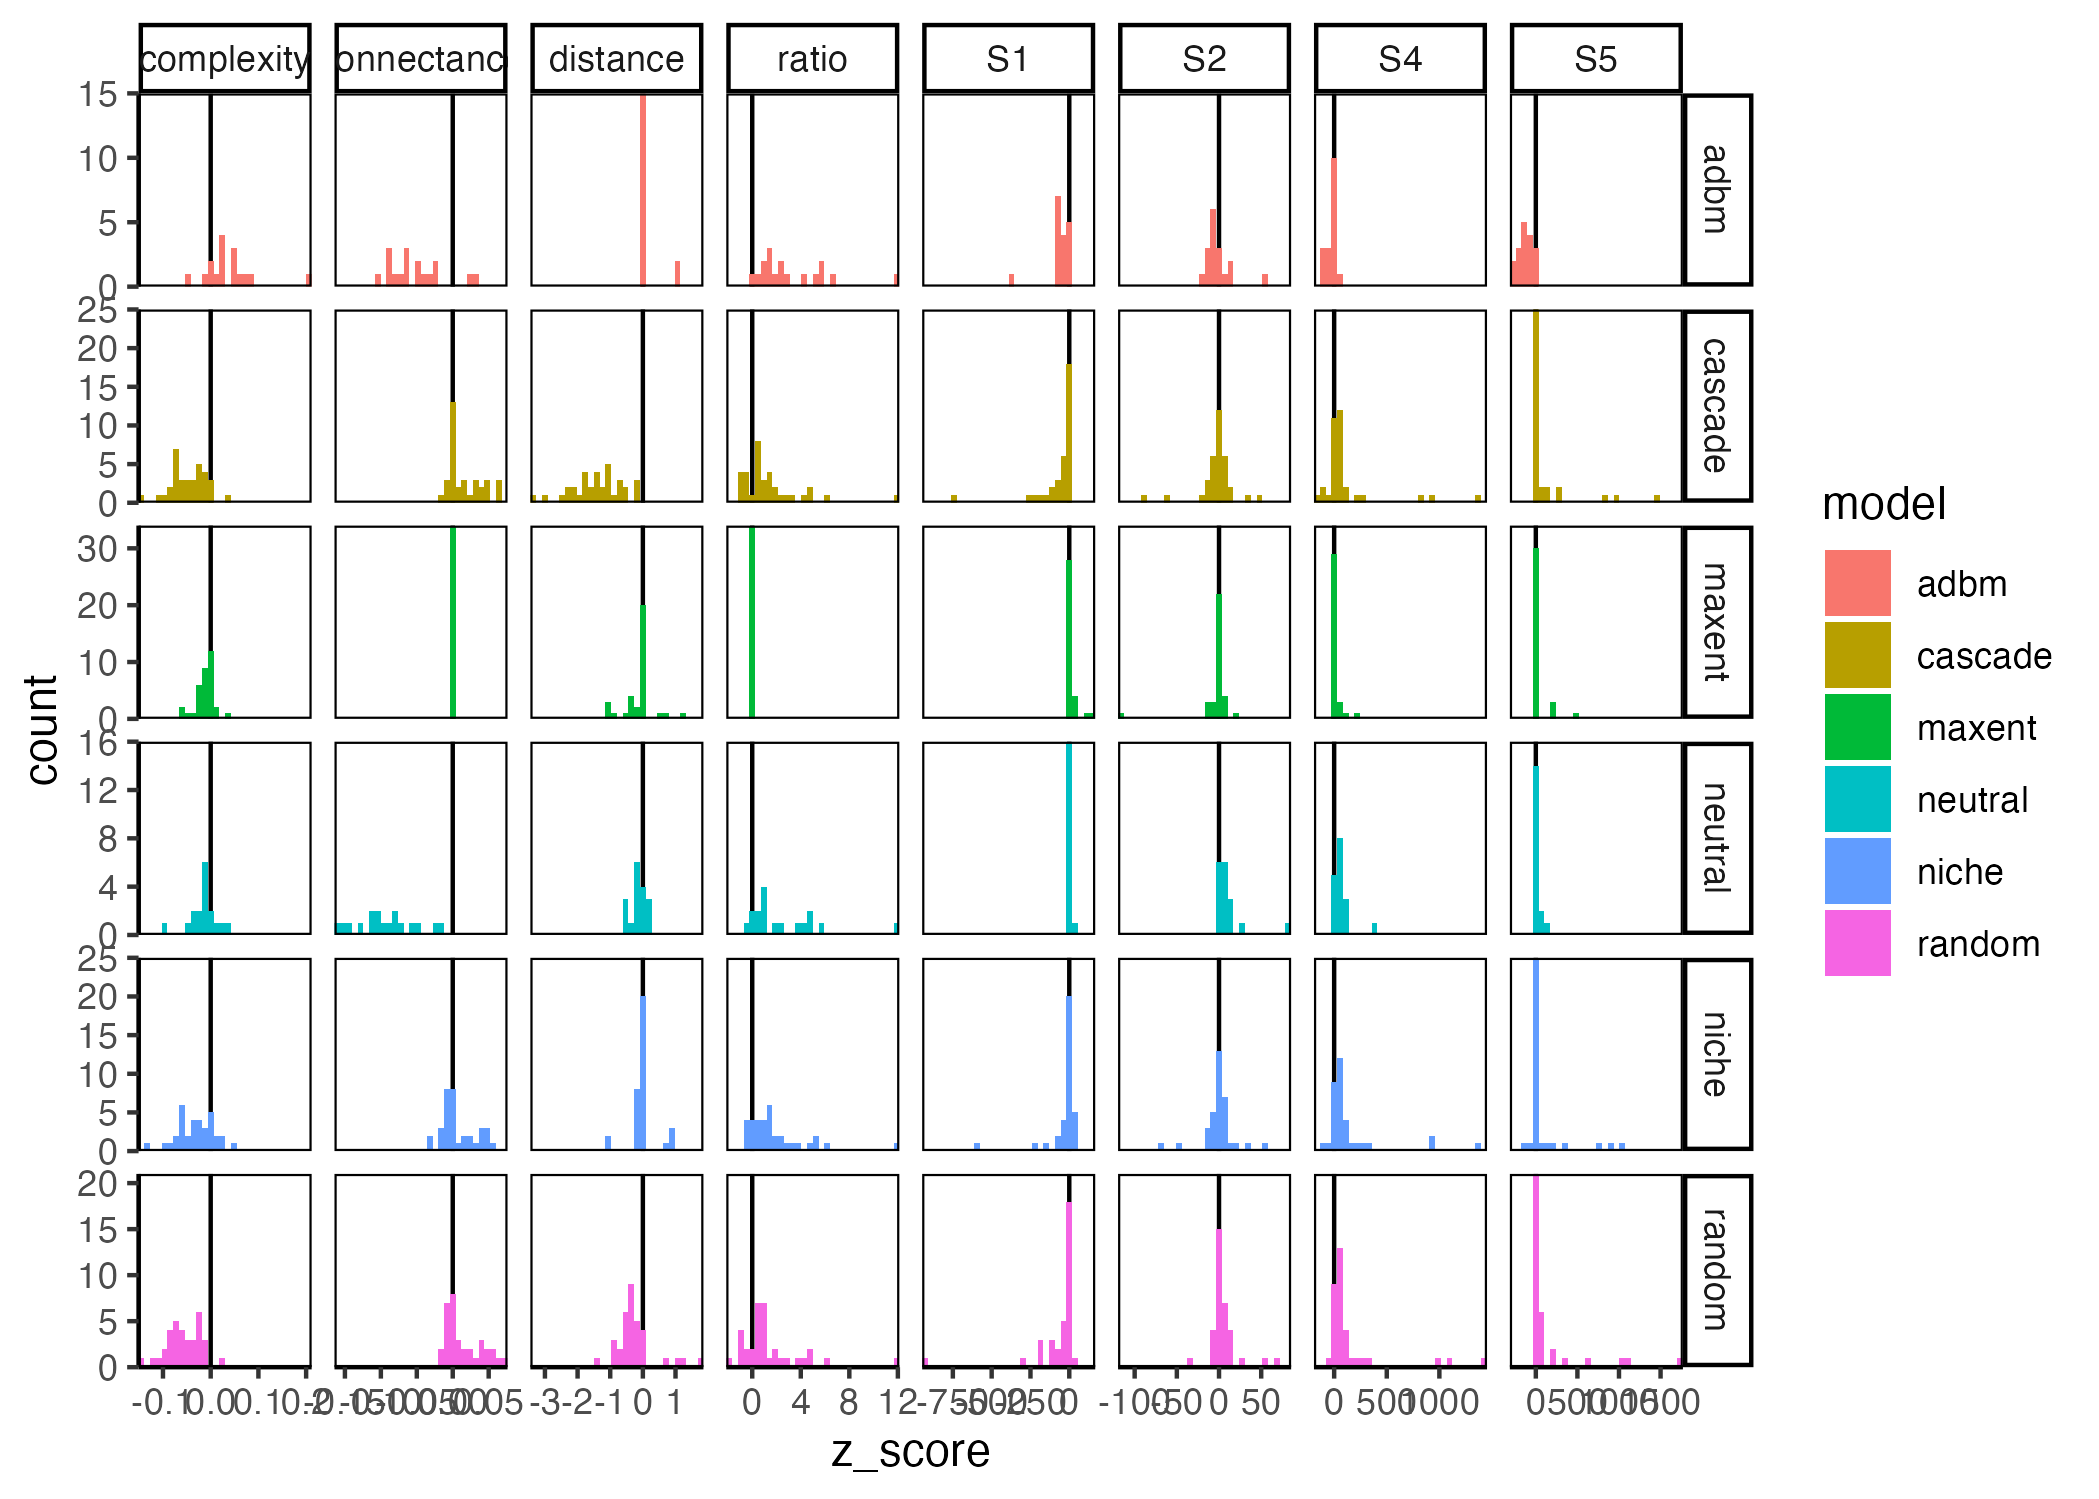
\includegraphics{images/topology.png}

}

\caption{\label{fig-topology}Difference between real and model network
property. S1 - S5 represent the different motif structures identified in
Stouffer et al. (2007) which are S1: Number of linear chains, S2: Number
of omnivory motifs, S4: Number of apparent competition motifs, and S5:
Number of direct competition motifs}

\end{figure}%

\textbf{Data cost}

This includes thinking about the need for additional data sources (such
as trait or phylogenetic data), the computational cost, as well as the
time it might take to generate a network, \emph{e.g.,} binary
classifiers require an (often times) extensive list of additional trait
data for the model training process, which limits predictions to
communities for which you do have the relevant auxiliary data available.

\textbf{Philosophical constraints}

Probably mentioned elsewhere but basically are we constructing networks
because we want to make real-world, case-specific predictions
\emph{e.g.,} for a conservation area or do we want to just have a set of
ecologically plausible networks we can use for theoretical stuffs. Need
to discuss the key differences and implications between predicting a
\textbf{metaweb} (\emph{sensu} Dunne (2006)) and a network realisation.
(In a way the idea of predicting a metaweb vs realisation is what makes
me hesitant to use the Mangal networks to test the structural models
because do we even know what the Mangal networks represent and what the
structural models are predicting\ldots) Maybe also Poisot et al. (2015)
that discuss how the local factors are going to play a role.

Also need to take into consideration inherent constraints that the model
imposes on itself and how it will affect our ability to test
hypotheses/ask questions using the \emph{e.g.,} from Petchey et al.
(2011) - models that are constrained by connectance means that we are
unable to explain connectance itself and you would need a different
approach if understanding connectance is your goal. Another way of
phrasing this is thinking about what is needed (input data/parameters),
produced (final network characteristics), and desired (end-use).

\begin{quote}
An interesting thing to also think about is data dependant and data
independent `parametrisation' of the models\ldots{}
\end{quote}

\end{tcolorbox}

\section{Concluding remarks}\label{concluding-remarks}

\begin{itemize}
\item
  As discussion about the different model families and in what areas
  they do/do not do well. This will depend probably a fair bit on how
  Figure~\ref{fig-topology} end up looking\ldots{} But it will also be
  important to tie in some of the other considerations/constraints that
  are listed in what is currently Box 2

  \begin{itemize}
  \tightlist
  \item
    In certain situations structure is `enough' but there may be use
    cases where we are really interested in the node-level interactions
    \emph{i.e.,} species identity is a thing we care about and need to
    be able to retrieve specific interactions at specific nodes
    correctly.
  \end{itemize}
\item
  Why do interaction models do so badly at predicting structure? Nuance
  of metaweb vs realisation but also time? At the core of it interaction
  models are trained on existing interaction data; this is data that are
  most likely closer to a metaweb than a local realisation even if they
  are being inventoried at a small scale\ldots{}

  \begin{itemize}
  \tightlist
  \item
    We can briefly shoehorn downsampling here maybe??
  \end{itemize}
\item
  It will be interesting to bring up the idea that if a model is missing
  a specific pairwise link but doing well overall then when does it
  matter?

  \begin{itemize}
  \item
    The fact that \emph{some} people are concerned about the taxonomic
    resolution and cascading effects those might have on our
    understanding of network structure (Pringle, 2020; Pringle \&
    Hutchinson, 2020), but that puts us in a place where we are at risk
    of losing our ability to distinguish the wood from the tree - are we
    not (at least at times) concerned more with understanding ecosystem
    level processes than with needing to understand things
    \emph{perfectly} at the species level.
  \item
    I don't think these `rare'/nuanced links (e.g.~carnivorous hippos)
    are going to rock the boat when we think about networks at the
    structural level.
  \end{itemize}
\end{itemize}

\begin{quote}
``The resolution of food-web data is demonic because it can radically
change network topology and associated biological inferences in ways
that are unknowable in the absence of better data.'' - Pringle \&
Hutchinson (2020) The counter to this is that structural models are
often not working at the species level and thus the structure remains
`unchanged' when you increase the resolution - I don't think that people
are that concerned with the structure of real world networks barring
connectance and since that scales with species richness anyway your
final proportion will probably still remain the same\ldots{}
\end{quote}

\begin{itemize}
\item
  I think a big take home will (hopefully) be how different approaches
  do better in different situations and so you as an end user need to
  take this into consideration and pick accordingly. I think Petchey et
  al. (2011) might have (and share) some thoughts on this. I feel like I
  need to look at Berlow et al. (2008) but maybe not exactly in this
  context but vaguely adjacent.

  \begin{itemize}
  \tightlist
  \item
    I think this is sort of the crux of the argument presented in
    Brimacombe et al. (2024) as well.
  \end{itemize}
\end{itemize}

\begin{quote}
\emph{``we highlight an interesting paradox: the models with the best
performance measures are not necessarily the models with the closest
reconstructed network structure.''} - Poisot (2023)
\end{quote}

\begin{itemize}
\item
  Do we need network models to predict interactions and interaction
  models to predict structure?

  \begin{itemize}
  \item
    ``Another argument for the joint prediction of networks and
    interactions is to reduce circularity and biases in the predictions.
    As an example, models like linear filtering generate probabilities
    of non-observed interactions existing, but do so based on measured
    network properties.'' - Strydom et al. (2021)
  \item
    Aligning (dove-tailing) with this the idea of ensemble modelling as
    presented by Becker et al. (2022)
  \end{itemize}
\item
  Close out with a call to action that we have models that predict
  networks very well and models that predict interactions very well but
  nothing that is doing well at predicting both - this is where we
  should be focusing our attention when it comes to furthering model
  development\ldots{}
\end{itemize}

\subsection{Downsampling}\label{downsampling}

do we bring this up? this could be a box\ldots{} if we have the
`finances' for it\ldots{} otherwise it should go to the outstanding
questions fur sure

\begin{itemize}
\item
  Dansereau et al. (2023)
\item
  ``That being said, there is a compelling argument for the need to
  `combine' these smaller functional units with larger spatial networks
  (Fortin et al., 2021) and that we should also start thinking about the
  interplay of time and space (Estay et al., 2023). Although deciding
  exactly what measure might actually be driving differences between
  local networks and the regional metaweb might not be that simple
  (Saravia et al., 2022).''
\end{itemize}

\section*{Glossary}\label{glossary}
\addcontentsline{toc}{section}{Glossary}

\begin{longtable}[]{@{}
  >{\raggedright\arraybackslash}p{(\columnwidth - 2\tabcolsep) * \real{0.5000}}
  >{\raggedright\arraybackslash}p{(\columnwidth - 2\tabcolsep) * \real{0.5000}}@{}}
\toprule\noalign{}
\begin{minipage}[b]{\linewidth}\raggedright
Term
\end{minipage} & \begin{minipage}[b]{\linewidth}\raggedright
Definition
\end{minipage} \\
\midrule\noalign{}
\endhead
\bottomrule\noalign{}
\endlastfoot
food web & a representation of feeding links between species \\
topology generator & a model that predicts a network based on
assumptions of structure, this network is species agnostic in the sense
that it does not necessarily contain information at the node level \\
interaction predictor & a model that predicts species interactions,
these interactions can be used to construct a network but there are no
\emph{a priori} assumptions as that will constrain the network
structure \\
model & A tool that can be used to construct food webs, where the
resulting network is a representation of a real world network. Models
typically only capture specific elements of real world networks and are
intended to be used in specific settings \\
model family & A family of models that share an underlying philosophy
when it comes to the mapping, pragmatism, and reduction of a network.
Families have the same underlying philosophies and assumptions that
determine the links between nodes as well as how these may be encoded \\
metaweb & A network that represents \emph{all} the potential links
between species. Importantly these links will not necessarily all be
realised in a specific location for a specific time \\
realised network & A network that represents the links between species
that are occurring. These networks represent a very localised
network\ldots{} \\
potential feeding link & links that indicate that an interaction is
ecologically feasible but not realised \emph{per se} (a metaweb would
contain potential feeding links) \\
realised feeding link & links that indicate that the interaction is
realised `in the field'. (a realised network contains realised feeding
links) \\
confusion matrix & captures the number of true positives (interaction
predicted as present when it is present), false negatives (interaction
predicted as absent when it is present), false positives (interaction
predicted as present when it is absent), and true negatives (interaction
predicted as absent when it is absent) \\
\end{longtable}

\section*{Outstanding questions}\label{outstanding-questions}
\addcontentsline{toc}{section}{Outstanding questions}

\begin{itemize}
\item
  non-consumptive effects
\item
  can we develop a model that is both a topology generator as well as an
  interaction predictor?
\item
  how do we define the spatial and temporal `boundaries' of a network
\end{itemize}

\section*{References}\label{references}
\addcontentsline{toc}{section}{References}

\phantomsection\label{refs}
\begin{CSLReferences}{1}{0}
\bibitem[\citeproctext]{ref-allesinaGeneralModelFood2008}
Allesina, S., Alonso, D., \& Pascual, M. (2008). A {General Model} for
{Food Web Structure}. \emph{Science}, \emph{320}(5876), 658--661.
\url{https://doi.org/10.1126/science.1156269}

\bibitem[\citeproctext]{ref-barberanUsingNetworkAnalysis2012}
Barberán, A., Bates, S. T., Casamayor, E. O., \& Fierer, N. (2012).
Using network analysis to explore co-occurrence patterns in soil
microbial communities. \emph{The ISME Journal}, \emph{6}(2), 343--351.
\url{https://doi.org/10.1038/ismej.2011.119}

\bibitem[\citeproctext]{ref-beckerOptimisingPredictiveModels2022}
Becker, D. J., Albery, G. F., Sjodin, A. R., Poisot, T., Bergner, L. M.,
Chen, B., Cohen, L. E., Dallas, T. A., Eskew, E. A., Fagre, A. C.,
Farrell, M. J., Guth, S., Han, B. A., Simmons, N. B., Stock, M.,
Teeling, E. C., \& Carlson, C. J. (2022). Optimising predictive models
to prioritise viral discovery in zoonotic reservoirs. \emph{The Lancet
Microbe}, \emph{3}(8), e625--e637.
\url{https://doi.org/10.1016/S2666-5247(21)00245-7}

\bibitem[\citeproctext]{ref-berlowGoldilocksFactorFood2008}
Berlow, E. L., Brose, U., \& Martinez, N. D. (2008). The {``{Goldilocks}
factor''} in food webs. \emph{Proceedings of the National Academy of
Sciences}, \emph{105}(11), 4079--4080.
\url{https://doi.org/10.1073/pnas.0800967105}

\bibitem[\citeproctext]{ref-berlowInteractionStrengthsFood2004}
Berlow, E. L., Neutel, A.-M., Cohen, J. E., de Ruiter, P. C., Ebenman,
B., Emmerson, M., Fox, J. W., Jansen, V. A. A., Iwan Jones, J.,
Kokkoris, G. D., Logofet, D. O., McKane, A. J., Montoya, J. M., \&
Petchey, O. (2004). Interaction strengths in food webs: Issues and
opportunities. \emph{Journal of Animal Ecology}, \emph{73}(3), 585--598.
\url{https://doi.org/10.1111/j.0021-8790.2004.00833.x}

\bibitem[\citeproctext]{ref-bhatiaNetworkbasedRestorationStrategies2023}
Bhatia, U., Dubey, S., Gouhier, T. C., \& Ganguly, A. R. (2023).
Network-based restoration strategies maximize ecosystem recovery.
\emph{Communications Biology}, \emph{6}(1), 1--10.
\url{https://doi.org/10.1038/s42003-023-05622-3}

\bibitem[\citeproctext]{ref-brimacombeApplyingMethodIts2024}
Brimacombe, C., Bodner, K., \& Fortin, M.-J. (2024). \emph{Applying a
method before its proof-of-concept: {A} cautionary tale using inferred
food webs}. \url{https://doi.org/10.13140/RG.2.2.22076.65927}

\bibitem[\citeproctext]{ref-brimacombeShortcomingsReusingSpecies2023}
Brimacombe, C., Bodner, K., Michalska-Smith, M., Poisot, T., \& Fortin,
M.-J. (2023). Shortcomings of reusing species interaction networks
created by different sets of researchers. \emph{PLOS Biology},
\emph{21}(4), e3002068.
\url{https://doi.org/10.1371/journal.pbio.3002068}

\bibitem[\citeproctext]{ref-caronTraitmatchingModelsPredict2024}
Caron, D., Brose, U., Lurgi, M., Blanchet, F. G., Gravel, D., \&
Pollock, L. J. (2024). Trait-matching models predict pairwise
interactions across regions, not food web properties. \emph{Global
Ecology and Biogeography}, \emph{33}(4), e13807.
\url{https://doi.org/10.1111/geb.13807}

\bibitem[\citeproctext]{ref-cirtwillQuantitativeFrameworkInvestigating2019}
Cirtwill, A. R., Eklf, A., Roslin, T., Wootton, K., \& Gravel, D.
(2019). A quantitative framework for investigating the reliability of
empirical network construction. \emph{Methods in Ecology and Evolution},
\emph{10}(6), 902--911. \url{https://doi.org/10.1111/2041-210X.13180}

\bibitem[\citeproctext]{ref-cleggImpactIntraspecificVariation2018}
Clegg, T., Ali, M., \& Beckerman, A. P. (2018). The impact of
intraspecific variation on food web structure. \emph{Ecology},
\emph{99}(12), 2712--2720. \url{https://doi.org/10.1002/ecy.2523}

\bibitem[\citeproctext]{ref-cohenCommunityFoodWebs1990}
Cohen, J. E., Briand, F., \& Newman, C. (1990). \emph{Community {Food
Webs}: {Data} and {Theory}}. Springer-Verlag.

\bibitem[\citeproctext]{ref-dansereauSpatiallyExplicitPredictions2023}
Dansereau, G., Barros, C., \& Poisot, T. (2023). \emph{Spatially
explicit predictions of food web structure from regional level data}.

\bibitem[\citeproctext]{ref-dormannRisePossibleFall2023}
Dormann, C. F. (2023). The rise, and possible fall, of network ecology.
In \emph{Defining {Agroecology} -- {A Festschrift} for {Teja
Tscharntke}} (pp. 143--159.). Tredition.

\bibitem[\citeproctext]{ref-dunnSixthMassCoextinction2009}
Dunn, R. R., Harris, N. C., Colwell, R. K., Koh, L. P., \& Sodhi, N. S.
(2009). The sixth mass coextinction: Are most endangered species
parasites and mutualists? \emph{Proceedings. Biological Sciences},
\emph{276}(1670), 3037--3045.
\url{https://doi.org/10.1098/rspb.2009.0413}

\bibitem[\citeproctext]{ref-dunneNetworkStructureFood2006}
Dunne, J. A. (2006). The {Network Structure} of {Food Webs}. In J. A.
Dunne \& M. Pascual (Eds.), \emph{Ecological networks: {Linking}
structure and dynamics} (pp. 27--86). Oxford University Press.

\bibitem[\citeproctext]{ref-dunneCompilationNetworkAnalyses2008}
Dunne, J. A., Williams, R. J., Martinez, N. D., Wood, R. A., \& Erwin,
D. H. (2008). Compilation and {Network Analyses} of {Cambrian Food
Webs}. \emph{PLOS Biology}, \emph{6}(4), e102.
\url{https://doi.org/10.1371/journal.pbio.0060102}

\bibitem[\citeproctext]{ref-estayEditorialPatternsProcesses2023}
Estay, S. A., Fortin, M.-J., \& López, D. N. (2023). Editorial:
{Patterns} and processes in ecological networks over space.
\emph{Frontiers in Ecology and Evolution}, \emph{11}.

\bibitem[\citeproctext]{ref-fortinNetworkEcologyDynamic2021}
Fortin, M.-J., Dale, M. R. T., \& Brimacombe, C. (2021). Network ecology
in dynamic landscapes. \emph{Proceedings of the Royal Society B:
Biological Sciences}, \emph{288}(1949), rspb.2020.1889, 20201889.
\url{https://doi.org/10.1098/rspb.2020.1889}

\bibitem[\citeproctext]{ref-hortalSevenShortfallsThat2015}
Hortal, J., de Bello, F., Diniz-Filho, J. A. F., Lewinsohn, T. M., Lobo,
J. M., \& Ladle, R. J. (2015). Seven {Shortfalls} that {Beset
Large-Scale Knowledge} of {Biodiversity}. \emph{Annual Review of
Ecology, Evolution, and Systematics}, \emph{46}(1), 523--549.
\url{https://doi.org/10.1146/annurev-ecolsys-112414-054400}

\bibitem[\citeproctext]{ref-hubbellUnifiedNeutralTheory2001}
Hubbell, S. P. (2001). \emph{The {Unified Neutral Theory} of
{Biodiversity} and {Biogeography} ({MPB-32})}. Princeton University
Press. \url{https://www.jstor.org/stable/j.ctt7rj8w}

\bibitem[\citeproctext]{ref-jordanoChasingEcologicalInteractions2016}
Jordano, P. (2016a). Chasing {Ecological Interactions}. \emph{PLOS
Biology}, \emph{14}(9), e1002559.
\url{https://doi.org/10.1371/journal.pbio.1002559}

\bibitem[\citeproctext]{ref-jordanoSamplingNetworksEcological2016}
Jordano, P. (2016b). Sampling networks of ecological interactions.
\emph{Functional Ecology}. \url{https://doi.org/10.1111/1365-2435.12763}

\bibitem[\citeproctext]{ref-lindemanTrophicDynamicAspectEcology1942}
Lindeman, R. L. (1942). The {Trophic-Dynamic Aspect} of {Ecology}.
\emph{Ecology}, \emph{23}(4), 399--417.
\url{https://doi.org/10.2307/1930126}

\bibitem[\citeproctext]{ref-morales-castillaInferringBioticInteractions2015}
Morales-Castilla, I., Matias, M. G., Gravel, D., \& Araújo, M. B.
(2015). Inferring biotic interactions from proxies. \emph{Trends in
Ecology \& Evolution}, \emph{30}(6), 347--356.
\url{https://doi.org/10.1016/j.tree.2015.03.014}

\bibitem[\citeproctext]{ref-petcheySizeForagingFood2008}
Petchey, O. L., Beckerman, A. P., Riede, J. O., \& Warren, P. H. (2008).
Size, foraging, and food web structure. \emph{Proceedings of the
National Academy of Sciences}, \emph{105}(11), 4191--4196.
\url{https://doi.org/10.1073/pnas.0710672105}

\bibitem[\citeproctext]{ref-petcheyFitEfficiencyBiology2011}
Petchey, O. L., Beckerman, A. P., Riede, J. O., \& Warren, P. H. (2011).
Fit, efficiency, and biology: {Some} thoughts on judging food web
models. \emph{Journal of Theoretical Biology}, \emph{279}(1), 169--171.
\url{https://doi.org/10.1016/j.jtbi.2011.03.019}

\bibitem[\citeproctext]{ref-pichlerMachineLearningAlgorithms2020}
Pichler, M., Boreux, V., Klein, A.-M., Schleuning, M., \& Hartig, F.
(2020). Machine learning algorithms to infer trait-matching and predict
species interactions in ecological networks. \emph{Methods in Ecology
and Evolution}, \emph{11}(2), 281--293.
\url{https://doi.org/10.1111/2041-210X.13329}

\bibitem[\citeproctext]{ref-poisotGuidelinesPredictionSpecies2023}
Poisot, T. (2023). Guidelines for the prediction of species interactions
through binary classification. \emph{Methods in Ecology and Evolution},
\emph{14}(5), 1333--1345. \url{https://doi.org/10.1111/2041-210X.14071}

\bibitem[\citeproctext]{ref-poisotGlobalKnowledgeGaps2021}
Poisot, T., Bergeron, G., Cazelles, K., Dallas, T., Gravel, D.,
MacDonald, A., Mercier, B., Violet, C., \& Vissault, S. (2021). Global
knowledge gaps in species interaction networks data. \emph{Journal of
Biogeography}, \emph{48}(7), 1552--1563.
\url{https://doi.org/10.1111/jbi.14127}

\bibitem[\citeproctext]{ref-poisotStructureProbabilisticNetworks2016}
Poisot, T., Cirtwill, A., Cazelles, K., Gravel, D., Fortin, M.-J., \&
Stouffer, D. (2016). The structure of probabilistic networks.
\emph{Methods in Ecology and Evolution}, \emph{7}(3), 303--312.
\url{https://doi.org/10}

\bibitem[\citeproctext]{ref-poisotSyntheticDatasetsCommunity2016}
Poisot, T., Gravel, D., Leroux, S., Wood, S. A., Fortin, M.-J., Baiser,
B., Cirtwill, A. R., Araújo, M. B., \& Stouffer, D. B. (2016). Synthetic
datasets and community tools for the rapid testing of ecological
hypotheses. \emph{Ecography}, \emph{39}(4), 402--408.
\url{https://doi.org/10.1111/ecog.01941}

\bibitem[\citeproctext]{ref-poisotSpeciesWhyEcological2015}
Poisot, T., Stouffer, D. B., \& Gravel, D. (2015). Beyond species: Why
ecological interaction networks vary through space and time.
\emph{Oikos}, \emph{124}(3), 243--251.
\url{https://doi.org/10.1111/oik.01719}

\bibitem[\citeproctext]{ref-poisotDescribeUnderstandPredict2016}
Poisot, T., Stouffer, D. B., \& Kéfi, S. (2016). Describe, understand
and predict: Why do we need networks in ecology? \emph{Functional
Ecology}, \emph{30}(12), 1878--1882.
\url{https://www.jstor.org/stable/48582345}

\bibitem[\citeproctext]{ref-pollockUnderstandingCooccurrenceModelling2014}
Pollock, L. J., Tingley, R., Morris, W. K., Golding, N., O'Hara, R. B.,
Parris, K. M., Vesk, P. A., \& McCarthy, M. A. (2014). Understanding
co-occurrence by modelling species simultaneously with a {Joint Species
Distribution Model} ({JSDM}). \emph{Methods in Ecology and Evolution},
\emph{5}(5), 397--406. \url{https://doi.org/10.1111/2041-210X.12180}

\bibitem[\citeproctext]{ref-pringleUntanglingFoodWebs2020}
Pringle, R. M. (2020). Untangling {Food Webs}. In \emph{Unsolved
{Problems} in {Ecology}} (pp. 225--238). Princeton University Press.
\url{https://doi.org/10.1515/9780691195322-020}

\bibitem[\citeproctext]{ref-pringleResolvingFoodWebStructure2020}
Pringle, R. M., \& Hutchinson, M. C. (2020). Resolving {Food-Web
Structure}. \emph{Annual Review of Ecology, Evolution and Systematics},
\emph{51}(Volume 51, 2020), 55--80.
\url{https://doi.org/10.1146/annurev-ecolsys-110218-024908}

\bibitem[\citeproctext]{ref-proulxNetworkThinkingEcology2005}
Proulx, S. R., Promislow, D. E. L., \& Phillips, P. C. (2005). Network
thinking in ecology and evolution. \emph{Trends in Ecology \&
Evolution}, \emph{20}(6), 345--353.
\url{https://doi.org/10.1016/j.tree.2005.04.004}

\bibitem[\citeproctext]{ref-saraviaEcologicalNetworkAssembly2022}
Saravia, L. A., Marina, T. I., Kristensen, N. P., De Troch, M., \& Momo,
F. R. (2022). Ecological network assembly: {How} the regional metaweb
influences local food webs. \emph{Journal of Animal Ecology},
\emph{91}(3), 630--642. \url{https://doi.org/10.1111/1365-2656.13652}

\bibitem[\citeproctext]{ref-shawFrameworkReconstructingAncient2024}
Shaw, J. O., Dunhill, A. M., Beckerman, A. P., Dunne, J. A., \& Hull, P.
M. (2024). \emph{A framework for reconstructing ancient food webs using
functional trait data} (p. 2024.01.30.578036). bioRxiv.
\url{https://doi.org/10.1101/2024.01.30.578036}

\bibitem[\citeproctext]{ref-staniczenkoStructuralDynamicsRobustness2010}
Staniczenko, P. P. A., Lewis, O. T., Jones, N. S., \& Reed-Tsochas, F.
(2010). Structural dynamics and robustness of food webs. \emph{Ecology
Letters}, \emph{13}(7), 891--899.
\url{https://doi.org/10.1111/j.1461-0248.2010.01485.x}

\bibitem[\citeproctext]{ref-stoufferEvidenceExistenceRobust2007}
Stouffer, D. B., Camacho, J., Jiang, W., \& Nunes Amaral, L. A. (2007).
Evidence for the existence of a robust pattern of prey selection in food
webs. \emph{Proceedings of the Royal Society B: Biological Sciences},
\emph{274}(1621), 1931--1940.
\url{https://doi.org/10.1098/rspb.2007.0571}

\bibitem[\citeproctext]{ref-strydomFoodWebReconstruction2022}
Strydom, T., Bouskila, S., Banville, F., Barros, C., Caron, D., Farrell,
M. J., Fortin, M.-J., Hemming, V., Mercier, B., Pollock, L. J., Runghen,
R., Dalla Riva, G. V., \& Poisot, T. (2022). Food web reconstruction
through phylogenetic transfer of low-rank network representation.
\emph{Methods in Ecology and Evolution}, \emph{13}(12), 2838--2849.
\url{https://doi.org/10.1111/2041-210X.13835}

\bibitem[\citeproctext]{ref-strydomGraphEmbeddingTransfer2023}
Strydom, T., Bouskila, S., Banville, F., Barros, C., Caron, D., Farrell,
M. J., Fortin, M.-J., Mercier, B., Pollock, L. J., Runghen, R., Dalla
Riva, G. V., \& Poisot, T. (2023). Graph embedding and transfer learning
can help predict potential species interaction networks despite data
limitations. \emph{Methods in Ecology and Evolution}, \emph{14}(12),
2917--2930. \url{https://doi.org/10.1111/2041-210X.14228}

\bibitem[\citeproctext]{ref-strydomRoadmapPredictingSpecies2021}
Strydom, T., Catchen, M. D., Banville, F., Caron, D., Dansereau, G.,
Desjardins-Proulx, P., Forero-Muñoz, N. R., Higino, G., Mercier, B.,
Gonzalez, A., Gravel, D., Pollock, L., \& Poisot, T. (2021). A roadmap
towards predicting species interaction networks (across space and time).
\emph{Philosophical Transactions of the Royal Society B: Biological
Sciences}, \emph{376}(1837), 20210063.
\url{https://doi.org/10.1098/rstb.2021.0063}

\bibitem[\citeproctext]{ref-thuillerNavigatingIntegrationBiotic2024}
Thuiller, W., Calderón-Sanou, I., Chalmandrier, L., Gaüzère, P.,
O'Connor, L. M. J., Ohlmann, M., Poggiato, G., \& Münkemüller, T.
(2024). Navigating the integration of biotic interactions in
biogeography. \emph{Journal of Biogeography}, \emph{51}(4), 550--559.
\url{https://doi.org/10.1111/jbi.14734}

\bibitem[\citeproctext]{ref-williamsSimpleRulesYield2000}
Williams, R. J., \& Martinez, N. D. (2000). Simple rules yield complex
food webs. \emph{Nature}, \emph{404}(6774), 180--183.
\url{https://doi.org/10.1038/35004572}

\bibitem[\citeproctext]{ref-williamsSuccessItsLimits2008}
Williams, R. J., \& Martinez, N. D. (2008). Success and its limits among
structural models of complex food webs. \emph{Journal of Animal
Ecology}, \emph{77}(3), 512--519.
\url{https://doi.org/10.1111/j.1365-2656.2008.01362.x}

\bibitem[\citeproctext]{ref-yeakelCollapseEcologicalNetwork2014}
Yeakel, J. D., Pires, M. M., Rudolf, L., Dominy, N. J., Koch, P. L.,
Guimarães, P. R., \& Gross, T. (2014). Collapse of an ecological network
in {Ancient Egypt}. \emph{PNAS}, \emph{111}(40), 14472--14477.
\url{https://doi.org/10.1073/pnas.1408471111}

\end{CSLReferences}




\end{document}
